\section{小结}

在当今数字化时代,人工智能生成内容(AIGC)正以前所未有的速度改变着我们的工作和学习方式。本章通过展示AIGC在文本、图像、音频和视频等多种形式内容生成中的应用,揭示了其强大的创造力和实用性。AIGC不仅能够快速生成高质量的内容,还能根据用户需求进行个性化定制,极大地提高了工作效率和学习效果。例如,通过自然语言处理技术,AIGC可以生成流畅且富有逻辑的文本,帮助用户快速撰写报告、文章或创意文案;在视觉艺术领域,它能够根据简单的描述生成精美的图像和设计,为设计师提供灵感;在音频和视频创作中,AIGC可以生成背景音乐、语音旁白甚至完整的视频内容,为多媒体制作开辟了新的可能性。这些应用不仅为专业人士提供了强大的工具,也为普通用户降低了创作门槛,使其能够轻松参与到内容创作中。然而,AIGC的发展也带来了版权、伦理和真实性等挑战,需要我们在使用过程中谨慎对待。随着技术的不断进步,AIGC将继续拓展其应用边界,成为未来工作和学习中不可或缺的助手。最终,AIGC将以AI agent的形式融入我们的日常生活,如\reffig{fig:ai-agent}所示,成为我们高效工作和深度学习的得力伙伴。

\fig[h]{
    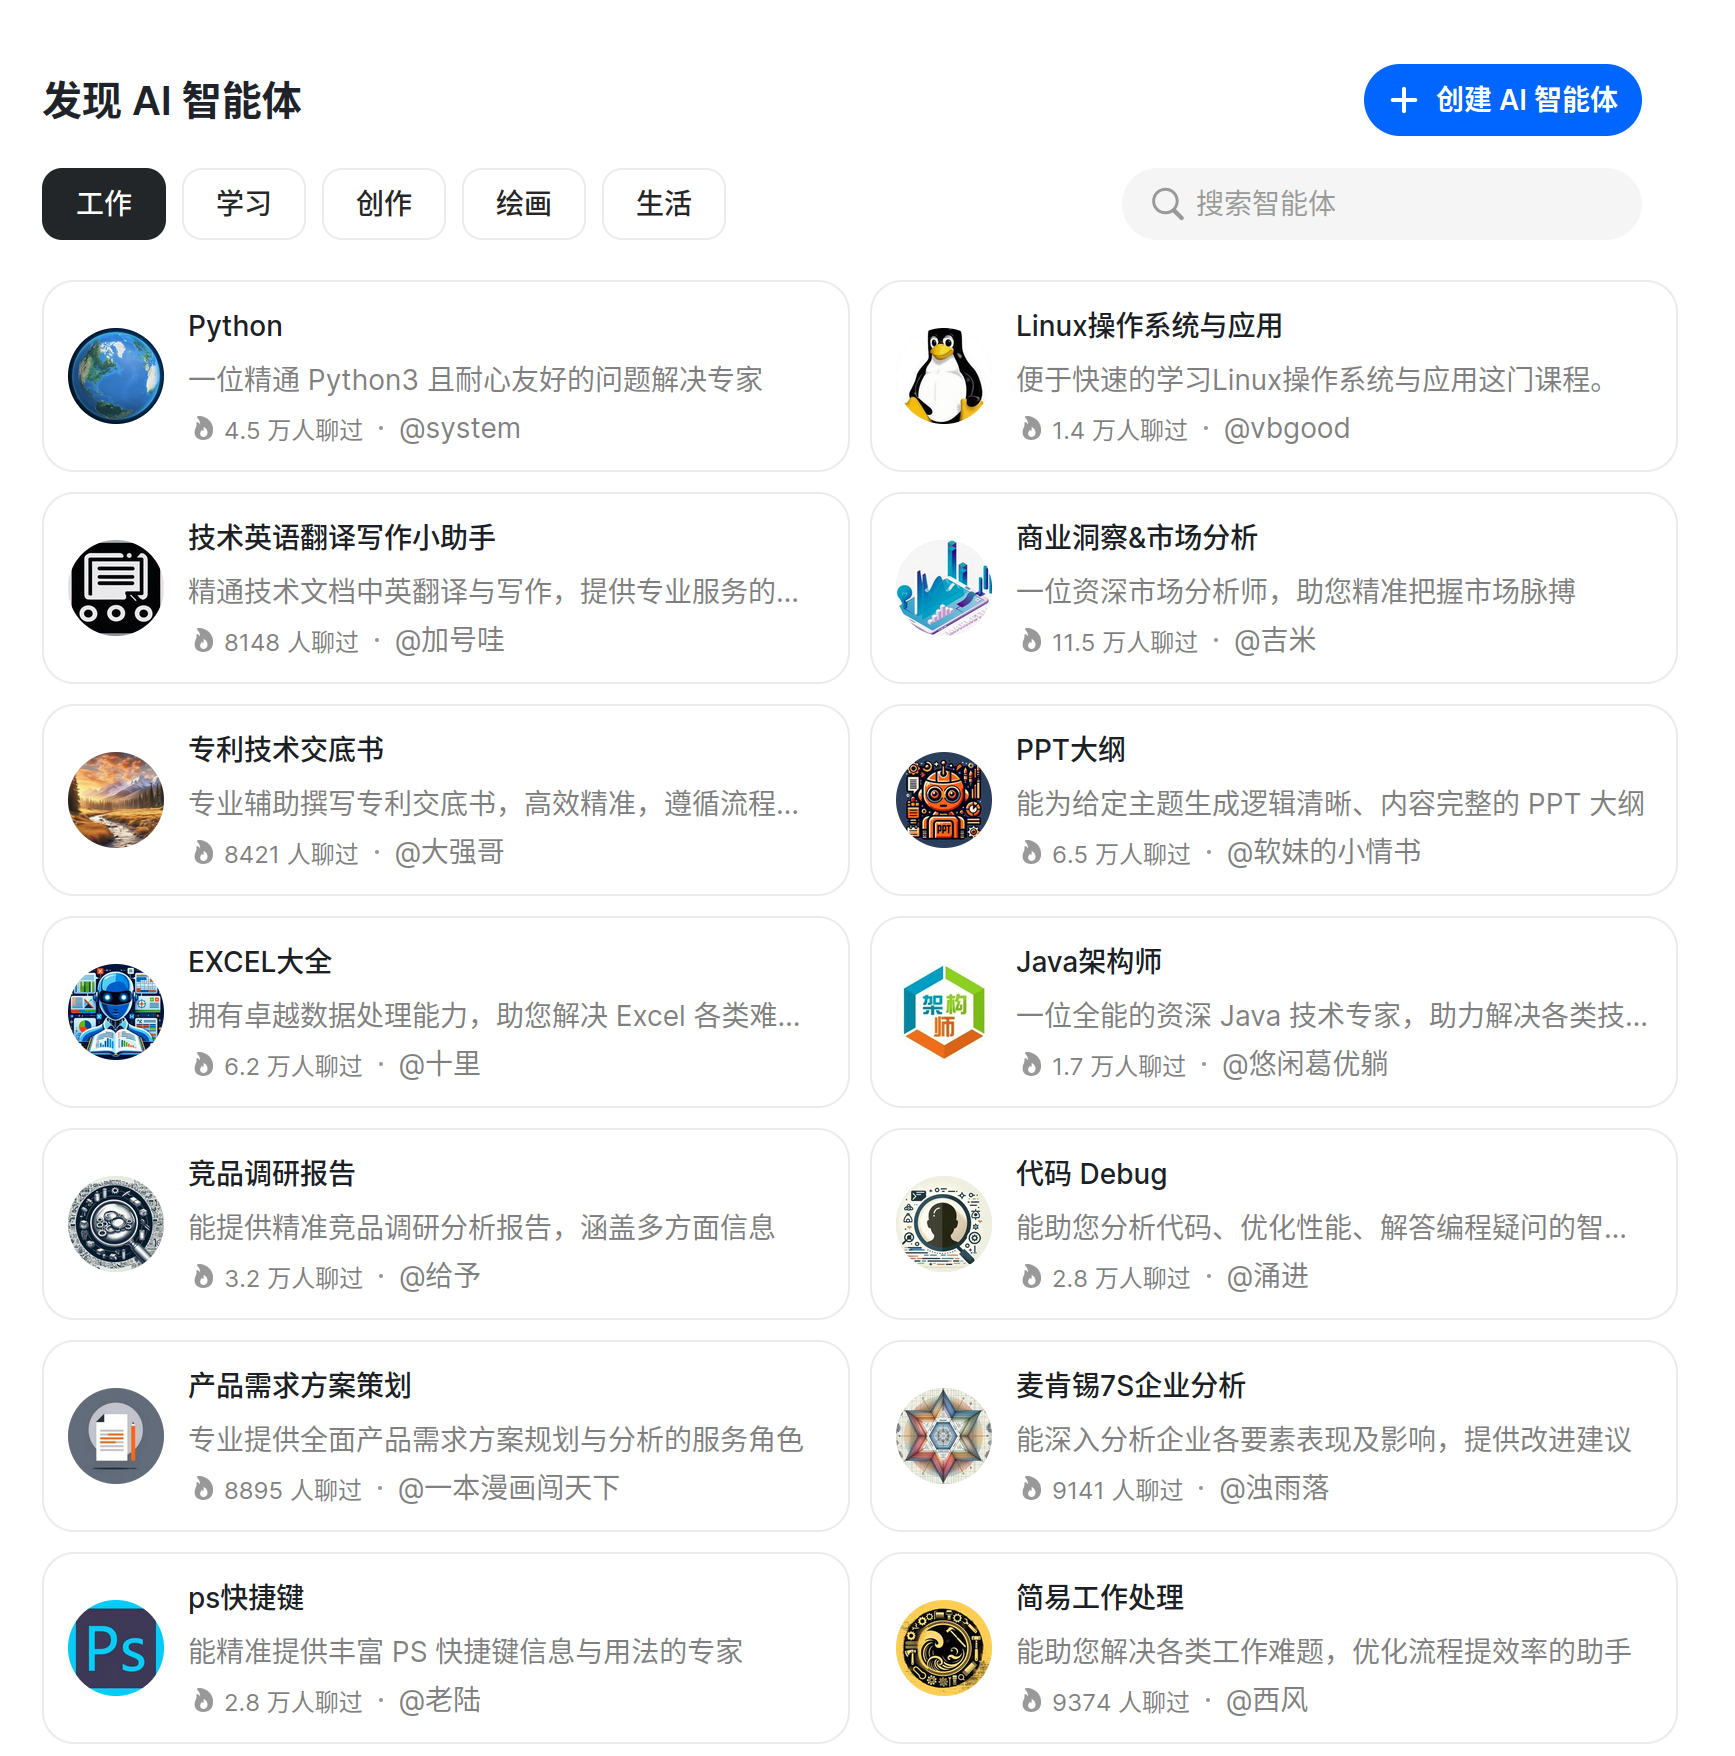
\includegraphics[width=0.7\textwidth]{ai_agent}
    \caption{AI Agent}
    \label{fig:ai-agent}
}